\subsection{Ejecución de la recursión}

Aprovechamos la sucesión de Fibonacci para estudiar cómo ejecuta una función recursiva.

\subsubsection{Árbol de ejecución}

Cada vez que se invoca \inline{fibonacci}, durante su ejecución se invoca nuevamente \inline{fibonacci} 0 o 2 veces. La manera convencional de representar ese mecanismo es mediante un \emph{árbol de ejecución} en el que cada nodo representa un llamado a la función y sus hijos son los llamados recursivos que hace. Para \inline{fibonacci(4)}:
\begin{center}
\begin{forest}
  for tree={
    draw, rounded corners,
    font=\ttfamily\small,
    inner sep=4pt,
    l sep=1.5em,
    s sep=1.2em,
    edge={-latex},
  }
  [{fibonacci(4)}
    [{fibonacci(3)}
      [{fibonacci(2)}
        [{fibonacci(1)}]
        [{fibonacci(0)}]
      ]
      [{fibonacci(1)}]
    ]
    [{fibonacci(2)}
      [{fibonacci(1)}]
      [{fibonacci(0)}]
    ]
  ]
\end{forest}
\end{center}
Nótese que, para toda función recursiva, el árbol de ejecución tiene las siguientes propiedades:
\begin{itemize}
  \item La raíz del árbol representa la invocación inicial de la función. Por ende, el árbol completo representa la solución del problema original.
  \item Cada nodo representa una invocación de la función, por lo que el conteo de nodos equivale al total de llamados.\item Cada subárbol representa entonces la solución de uno de los subproblemas y la cantidad de subárboles el número de subproblemas.
  \item Los hijos representan las llamadas recursivas realizadas por esa invocación. 
  \begin{itemize}
    \item En el caso de \inline{fibonacci}, siempre se realizan 0 o 2 llamados, por lo cual cada nodo tiene 0 o 2 hijos. Eso resulta en un árbol binario.
  \end{itemize}
  \item Los hojas representan entonces llamados de la función en los que no se realizan llamados recursivos, es decir, en los que se alcanza el caso base.
\end{itemize}

\subsubsection{Orden de ejecución}

Al leer un programa iterativo, el orden de ejecución coincide con el orden textual del código: de arriba hacia abajo, repetidamente. Esto no sucede en la recursión, por lo que vale la pena ahondar en cómo entender el orden de los llamados.

Supóngase que se invoca \inline{fibonacci(4)}. El código salta el caso base y llega directamente a la línea de retorno, pero antes de retornar ejecuta el lado izquierdo de la suma, \inline{fibonacci(3)}. Inmediatamente entra en el contexto de ese llamado, antes de ejecutar el lado derecho de la suma. Por ende, todos los llamados recursivos dentro de \inline{fibonacci(3)} ejecutan antes que el lado derecho de la suma; luego todos los llamados recursivos del lado derecho de la suma ejecutan; y, de últimas, en efecto ocurre la suma y termina la ejecución de \inline{fibonacci(4)}.

El árbol de ejecución no enfatiza en el orden en el que se realizan los llamados, por lo que el siguiente grafo dirigido añade aristas numeradas que ilustran el orden de ejecución. Como los hijos son invocados por los padres, las aristas dirigidas hacia abajo denotan que una función invoca a otra; se ilustran en azul. Las aristas dirigidas hacia arriba denotan que la función invocada retorna a la que la invocó y se ilustran en verde.

\begin{center}
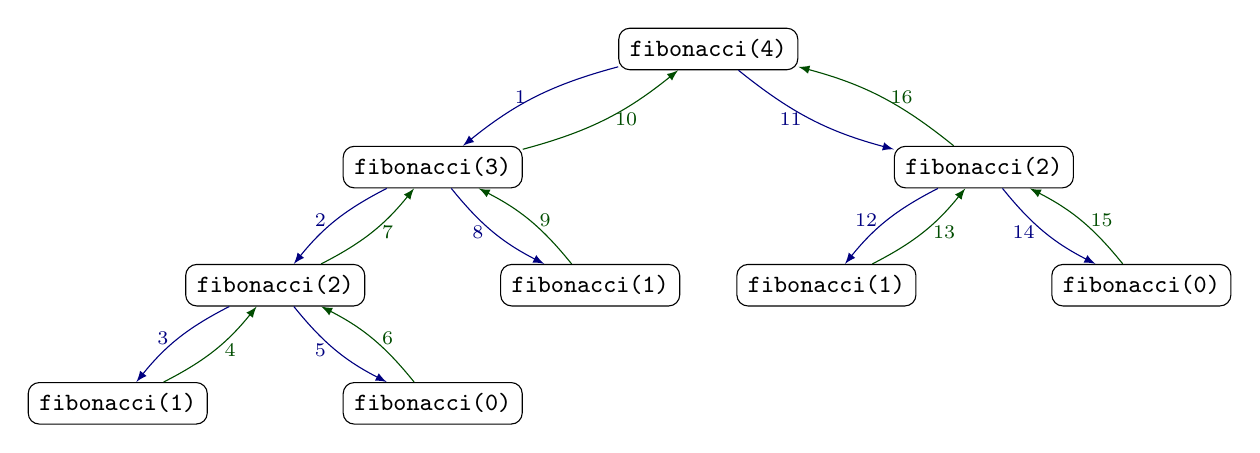
\begin{tikzpicture}[
  box/.style={draw, rounded corners, font=\small\ttfamily, inner sep=4pt},
  call/.style={-latex, blue!50!black, bend right=12},
  ret/.style={-latex, green!30!black, bend right=12},
]
  \node[box] (f4)  at ( 0,     0) {fibonacci(4)};
  \node[box] (f3)  at (-3.5,-1.5) {fibonacci(3)};
  \node[box] (f2b) at ( 3.5,-1.5) {fibonacci(2)};
  \node[box] (f2a) at (-5.5,  -3) {fibonacci(2)};
  \node[box] (f1b) at (-1.5,  -3) {fibonacci(1)};
  \node[box] (f1c) at ( 1.5,  -3) {fibonacci(1)};
  \node[box] (f0b) at ( 5.5,  -3) {fibonacci(0)};
  \node[box] (f1a) at (-7.5,-4.5) {fibonacci(1)};
  \node[box] (f0a) at (-3.5,-4.5) {fibonacci(0)};

  \draw[call] (f4)  to node[left,  font=\scriptsize] {1}  (f3);
  \draw[call] (f4)  to node[left,  font=\scriptsize] {11} (f2b);
  \draw[call] (f3)  to node[left,  font=\scriptsize] {2}  (f2a);
  \draw[call] (f3)  to node[left,  font=\scriptsize] {8}  (f1b);
  \draw[call] (f2b) to node[left,  font=\scriptsize] {12} (f1c);
  \draw[call] (f2b) to node[left,  font=\scriptsize] {14} (f0b);
  \draw[call] (f2a) to node[left,  font=\scriptsize] {3}  (f1a);
  \draw[call] (f2a) to node[left,  font=\scriptsize] {5}  (f0a);

  \draw[ret] (f3)  to node[right, font=\scriptsize] {10} (f4);
  \draw[ret] (f2b) to node[right, font=\scriptsize] {16} (f4);
  \draw[ret] (f2a) to node[right, font=\scriptsize] {7}  (f3);
  \draw[ret] (f1b) to node[right, font=\scriptsize] {9}  (f3);
  \draw[ret] (f1c) to node[right, font=\scriptsize] {13} (f2b);
  \draw[ret] (f0b) to node[right, font=\scriptsize] {15} (f2b);
  \draw[ret] (f1a) to node[right, font=\scriptsize] {4}  (f2a);
  \draw[ret] (f0a) to node[right, font=\scriptsize] {6}  (f2a);
\end{tikzpicture}
\end{center}

Como al invocar una función esta ejecuta de forma inmediata, la ejecución recursiva siempre explora completamente una rama del árbol antes de pasar a la siguiente. Con eso en mente y observando el flujo de ejecución expuesto arriba, se puede ver que el orden de ejecución de toda función recursiva está dado por un recorrido DFS %TODO: Hyperlink/ref!!
sobre el árbol de ejecución.

\subsubsection{Pila de ejecución}

La inmensa mayoría de las arquitecturas y entornos de ejecución modernos utilizan una \emph{pila de llamados} (\textit{call stack}) para administrar las llamadas a funciones. Se aprovecha la estructura LIFO (\textit{Last-In, First-Out}; última que entra, primera que sale) de la pila para que la última función en ser invocada termine primero.

Cuando una función $A$ llama a una función $B$, se crea un \emph{marco de pila} (\textit{stack frame}) con la información de $B$: sus parámetros, las variables locales y la dirección de retorno (la ubicación a la que debe volver la ejecución cuando $B$ termine). Al colocar el marco de pila de $B$ en la pila de llamadas, queda encima del marco de pila de $A$, que a su vez está encima del marco de pila de la función que la invocó. Así pues, la pila refleja en todo momento la cadena de llamadas activas. Cuando $B$ retorna, su marco se elimina de la pila y la ejecución continúa en $A$, donde indica la dirección de retorno.

Si una función se invoca recursivamente, cada llamada recursiva genera un nuevo marco de pila, a pesar de que cada llamado corresponda a la misma función y al mismo código fuente, pues las ejecuciones deben ser independientes. Los llamados se apilan en el orden en el que ocurren, es decir, de acuerdo con un recorrido DFS sobre el árbol de ejecución. A medida que terminan, se remueven de la pila. Por ende, en cada nodo del árbol, la profundidad de la pila (i.e., el número de marcos de pila que tiene) es igual a la distancia de ese nodo a la raíz. Una consecuencia de eso es que la máxima profundidad que alcanza la pila coincide con la altura del árbol de ejecución, que es la longitud de su camino más largo de raíz a hoja. Esa última observación es relevante para el cálculo de la complejidad espacial.